\subsubsection{Subsistema para los relés}\label{subsubsec:hardware/circuito-reles}

La selección de tensión de alimentación para los cargadores y la carga o descarga de la batería de \textit{Backup} se ha realizado mediante relés. Debido a la naturaleza del proyecto, es interesante reducir al mínimo posible el consumo de corriente de los elementos del circuito, por lo que el consumo constante de un relé no es algo admisible.

Se tuvo en consideración el uso de relés biestables, pero su elevado coste en comparación y la recomendación de realizar un subsistema electrónico con una PCB propia, decidimos tomar otra alternativa. 

La corriente que un relé necesita para conmutar es menor que la que necesita para mantener el interruptor conmutado, por lo que decidimos realizar un circuito que aplicara un pico de corriente al conmutar y reduejera la corriente para mantener la conmutación. 

Se puede ver el circuito en la \autoref{fig:hardware/modulos/reles/esquematico}. Se utiliza un condensador y una resistencia que consiguen una respuesta subamortiguada ante el escalón de conmutación. Además, se utiliza un transistor para manejar la conmutación del relé y se utiliza un diodo de \textit{flyback} para proteger a dicho transistor de la corriente de la bobina cuando se intente cortar. Para la resistencia en paralelo con el condensador se ha utilizado un potenciómetro para poder ajustar el pico de conmutación. 

\begin{figure}[H]
    \centering
    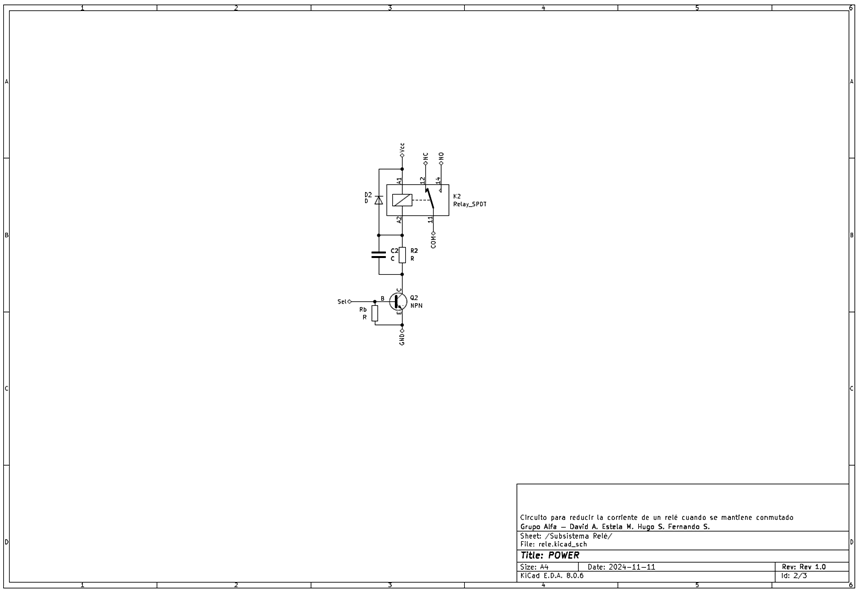
\includegraphics[width=0.5\textwidth]{images/2-hardware/componentes/rele/circuitoRele.png}
    \caption{Esquemático básico del circuito de los relés}
    \label{fig:hardware/modulos/reles/esquematico}
\end{figure}

El valor de los componentes pasivos se ha elegido experimentalmente, en función de los valores que mejores resultados han dado en el laboratorio. El propósito de cada componente es:
\begin{itemize}
    \item \texttt{R1}: Reduce la tensión aplicada en la bobina, ya que esta es de $12\ V$ y este circuito se puede alimentar con $24\ V$. Se ha utilizado un valor de $100\ \Omega$.
    \item \texttt{R2}: Potenciómetro que junto a \texttt{C1} crean la respuesta subamortiguada en la conmutación. Se ha utilizado un valor de $2.2\ k\Omega$.
    \item \texttt{R3}: Resistencia para limitar la corriente de base del transistor, ya que va a venir de un \texttt{GPIO} del microcontrolador. Se ha utilizado un valor de $100\ \Omega$.
    \item \texttt{R4}: Resistencia de \textit{pull-down} para colocar un nivel bajo débil en la base del transistor. Se ha utilizado un valor de $1\ k\Omega$.
    \item \texttt{C1}: Condensador utilizado para la respuesta subamortiguada del sistema. Inicialmente se encuentra descargado, por lo que actúa como un cortocircuito , creando el pico de corriente. Según se va cargando, va tomando importancia la resistencia y esta es la que decide la corriente final del relé. Se ha utilizado un valor de $1000\ \mu F$.
    \item \texttt{Q1}: Transistor encargado de la conmutación del relé. Es accionado desde un \texttt{GPIO} del microcontrolador. Se ha utilizado el transistor \texttt{PNP} modelo \texttt{2N2222}. 
    \item \texttt{D1}: Diodo de \textit{flyback} utilizado para redirigir la corriente de la bobina cuando se corta el transistor, para evitar destruirlo. Se ha utilizado un diodo \texttt{1N4007} por ser el más accesible, aunque lo óptimo hubiera sido un diodo Schottky.
\end{itemize}

Para el montaje de dicho circuito se ha diseñado una PCB que se ha enviado a fabricar a una empresa extranjera. El resulado se puede ver en la \autoref{fig:hardware/modulos/reles/fotoPCB}. Las resistencias soldadas en la imagen no tienen los valores indicados porque se cambiaron después de hacer la foto.

\begin{figure}[H]
    \centering
    \begin{subfigure}[b]{0.45\textwidth}
        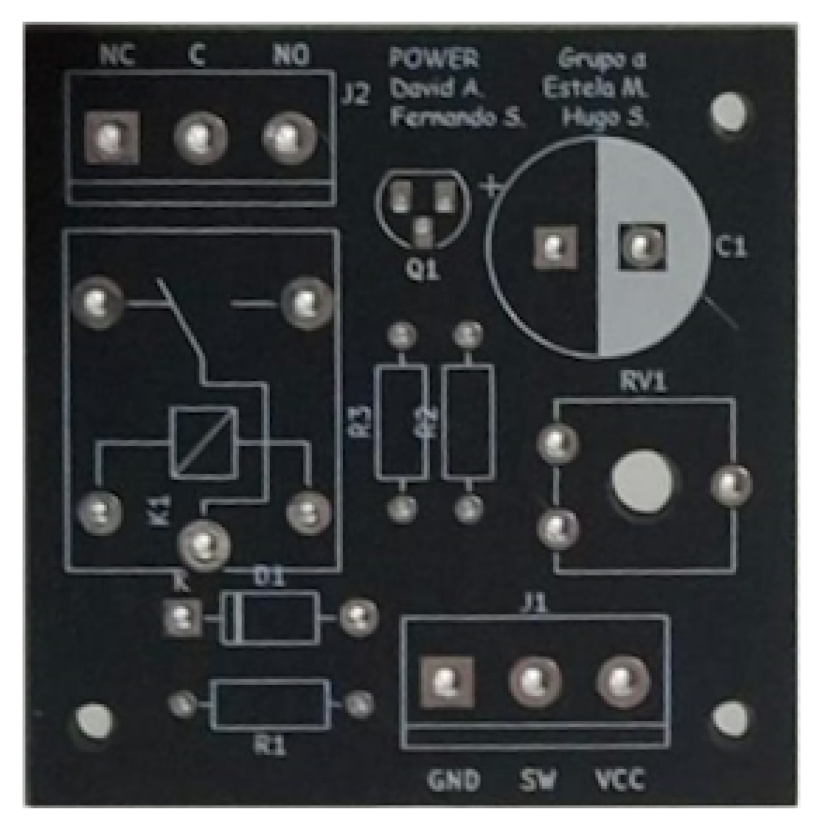
\includegraphics[width=\textwidth]{images/2-hardware/componentes/rele/pcbRele.png}
        \caption{PCB sin montar}
    \end{subfigure}
    \hfill
    \begin{subfigure}[b]{0.45\textwidth}
        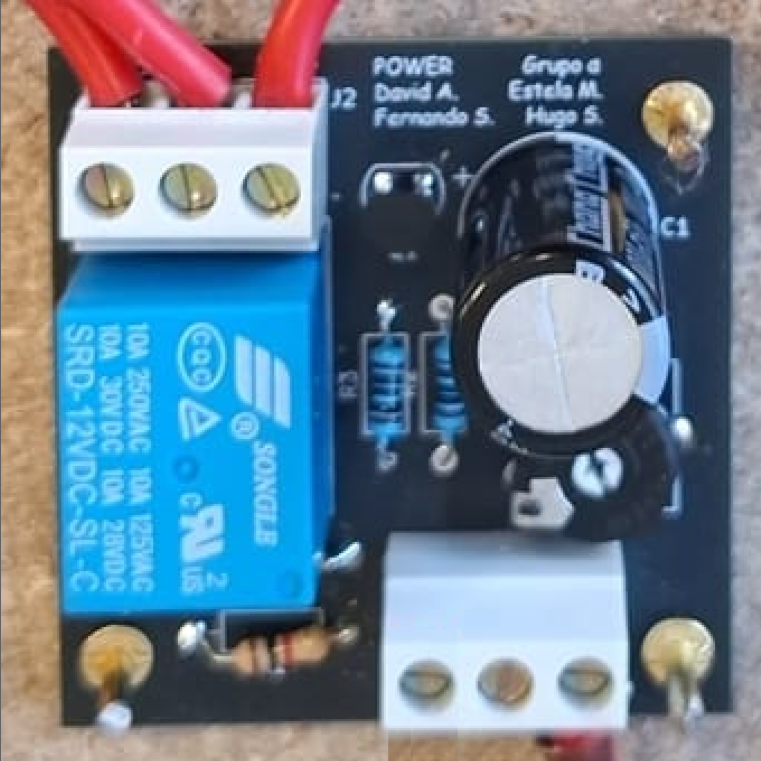
\includegraphics[width=\textwidth]{images/2-hardware/componentes/rele/pcbReleMontada.png}
        \caption{Circuito montado}
    \end{subfigure}
    \caption{PCB del circuito para los relés}
    \label{fig:hardware/modulos/reles/fotoPCB}
\end{figure}

Observando la forma de onda de la corriente de conmutación (proporcional a la tensión en la resistencia \texttt{R1}), se ve la diseñada respuesta subamortiguada.

\begin{figure}[H]
    \centering
    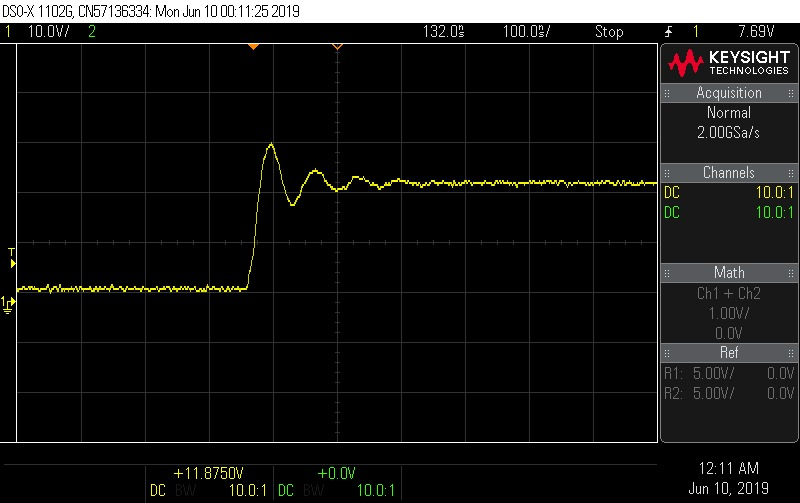
\includegraphics[width=0.5\textwidth]{images/2-hardware/componentes/rele/respuestaSubamortiguada.jpg}
    \caption{Respuesta subamortiguada del circuito del relé}
    \label{fig:hardware/reles/respuesta}
\end{figure}

Con este circuito alimentado a $24\ V$, se consigue reducir la corriente de un relé desde $60.2\ mA$ a $14.1\ mA$.